\documentclass[11pt,a4paper]{article}
\usepackage[utf8]{inputenc}
\usepackage[margin=2.2cm]{geometry}
\usepackage{amsmath,amssymb}
\usepackage{hyperref}
\usepackage{xcolor}
\usepackage{booktabs}
\usepackage{listings}
\usepackage{graphicx}
\usepackage{enumitem}
\usepackage{caption}
\usepackage{subcaption}
\usepackage{longtable}
\usepackage{microtype}
\usepackage{parskip}
\usepackage{textcomp}

\hypersetup{colorlinks=true,linkcolor=blue!50!black,urlcolor=blue!60!black}

\lstset{basicstyle=\ttfamily\footnotesize,breaklines=true,
        frame=single,framerule=0pt,backgroundcolor=\color{black!4},
        columns=fullflexible,keepspaces=true,
        showstringspaces=false,xleftmargin=0pt}

\title{Julia v1.5 SMC$^2$-MPC horizon sweep \\
       \large $T \in \{14, 28, 42, 56, 70, 84\}$ days, RTX 5090, seed 42}
\author{}
\date{2026-05-09}

\begin{document}
\maketitle

\begin{abstract}
This report records a six-horizon sweep of the FSA v1.5 closed-loop
SMC$^2$-MPC bench on the Julia stack at saturated configuration
\cite{techguide}. All flag values, output paths, headline numbers,
and per-horizon plots are included so the run can be reproduced
verbatim. The model SDE definition (\S\ref{sec:model}), the
SMC$^2$-MPC pipeline and cost (\S\ref{sec:smc2}), and the bench CLI
(\S\ref{sec:cli}) are sourced from the comparison writeup
\cite{writeup} and the technical guide \cite{techguide}; numerical
results in tables \ref{tab:gpu_timing}--\ref{tab:phi_summary} and
figures \ref{fig:traces_T14}--\ref{fig:param_T84} are sourced from
the run artefacts on disk.
\end{abstract}

\tableofcontents
\clearpage


% =====================================================================
\section{The FSA v1.5 model}
\label{sec:model}

\subsection{State variables}

FSA (Fitness--Stress--Autonomic) is a 3-state stochastic differential
equation model for an athlete's response to training. State
$y = (B, F, A)$:

\begin{itemize}[itemsep=2pt]
  \item $B$ --- aerobic fitness (Banister chronic; bounded $[0, 1]$,
        Jacobi-style state-dependent diffusion).
  \item $F$ --- unified fatigue (Banister acute; $\geq 0$, CIR-style
        diffusion).
  \item $A$ --- autonomic amplitude (Stuart--Landau; $\geq 0$, CIR-style
        diffusion).
\end{itemize}

\subsection{Drift}

In \texttt{/day} units:
\begin{align}
  \mu(B, F)        &= \mu_0 + \mu_B B - \mu_F F - \mu_{FF} F^2 \\
  dB/dt            &= \kappa_B \, (1 + \varepsilon_A A) \, \Phi(t) - B / \tau_B \\
  dF/dt            &= \kappa_F \, \Phi(t) - (1 + \lambda_A A) / \tau_F \, F \\
  dA/dt            &= \mu(B, F) \cdot A - \eta A^3
\end{align}

The single exogenous control is $\Phi(t)$, the training-strain rate
($\geq 0$).

\subsection{State-dependent diffusion (It\^o)}

\begin{align}
  \sigma_B(B) \, dW_B &= \sigma_B \sqrt{B(1-B)} \, dW_B  & \text{(Jacobi, $[0,1]$)} \\
  \sigma_F(F) \, dW_F &= \sigma_F \sqrt{F} \, dW_F        & \text{(CIR, $\geq 0$)} \\
  \sigma_A(A) \, dW_A &= \sigma_A \sqrt{A} \, dW_A        & \text{(CIR, $\geq 0$)}
\end{align}

The diffusion vanishes at each domain boundary so the SDE keeps the
state in its physiological range without clipping.

\subsection{Observation channels}

Three direct-Gaussian observation channels:
\begin{equation}
  y^{\mathrm{obs}}_B = B + \mathcal{N}(0, \sigma_{B,\mathrm{obs}}^2),
  \qquad
  y^{\mathrm{obs}}_F = F + \mathcal{N}(0, \sigma_{F,\mathrm{obs}}^2),
  \qquad
  y^{\mathrm{obs}}_A = A + \mathcal{N}(0, \sigma_{A,\mathrm{obs}}^2).
\end{equation}
No HR / sleep / stress / steps channels (that is the v2 surface). No
circadian forcing. All three obs noise scales pinned at $0.005$.

\subsection{Time grid}

60 minutes per bin (24 bins per day); $\Phi(t)$ is constant within a
bin. The closed-loop bench's stride is 12 bins (12 hours) and its
filter window is 24 bins (1 day).

\subsection{Parameters: 14 dynamics + 3 obs noise; 10 estimated, 7 pinned}

The 14 dynamics parameters use the v1.5 basis: $\kappa_B$ is replaced
by $B_\infty = \kappa_B \tau_B$ and $\kappa_F$ by
$F_\infty = \kappa_F \tau_F$ (steady-state fitness / fatigue at
$\Phi = 1$, no $A$-coupling) for better identifiability under the
direct-Gaussian observation model. The basis-rotation adapter is at
\texttt{simulation.params\_v15\_to\_v1\_nt} (Julia) /
\texttt{simulation.params\_v15\_to\_v1} (Python+JAX).

\begin{table}[ht]
\centering
\small
\begin{tabular}{lllrl}
\toprule
Symbol & Role & Truth value & Pinned & Prior (estimated only) \\
\midrule
$\tau_B$            & chronic-$B$ time constant   & 42.0    & yes & --- \\
$\tau_F$            & acute-$F$ time constant     & 7.0     & no  & LogNormal($\log 7.0,\ 0.30$) \\
$B_\infty$          & steady-state $B$ at $\Phi=1$ & 0.504   & no  & LogNormal($\log 0.504,\ 0.30$) \\
$F_\infty$          & steady-state $F$ at $\Phi=1$ & 0.21    & no  & LogNormal($\log 0.21,\ 0.30$) \\
$\varepsilon_A$     & $A$-on-$B$ multiplicative coupling & 0.40 & yes & --- \\
$\lambda_A$         & $A$-on-$F$ recovery coupling & 1.00    & no  & LogNormal($\log 1.0,\ 0.30$) \\
$\mu_0$             & Stuart--Landau bias         & 0.02    & no  & LogNormal($\log 0.02,\ 0.30$) \\
$\mu_B$             & SL slope on $B$             & 0.30    & no  & LogNormal($\log 0.30,\ 0.30$) \\
$\mu_F$             & SL slope on $F$             & 0.10    & no  & LogNormal($\log 0.10,\ 0.30$) \\
$\mu_{FF}$          & SL curvature on $F^2$       & 0.40    & yes & --- \\
$\eta$              & SL cubic damping            & 0.20    & yes & --- \\
$\sigma_B$          & dynamics noise scale on $B$ & 0.010   & no  & LogNormal($\log 0.010,\ 0.30$) \\
$\sigma_F$          & dynamics noise scale on $F$ & 0.012   & no  & LogNormal($\log 0.012,\ 0.30$) \\
$\sigma_A$          & dynamics noise scale on $A$ & 0.020   & no  & LogNormal($\log 0.020,\ 0.30$) \\
\midrule
$\sigma_{B,\mathrm{obs}}$ & obs noise on $B$ channel & 0.005 & yes & --- \\
$\sigma_{F,\mathrm{obs}}$ & obs noise on $F$ channel & 0.005 & yes & --- \\
$\sigma_{A,\mathrm{obs}}$ & obs noise on $A$ channel & 0.005 & yes & --- \\
\bottomrule
\end{tabular}
\caption{All 17 v1.5 parameters. 10 are estimated by the filter
(LogNormal priors centred on $\log(\text{truth})$ with scale $0.30$);
7 are pinned at truth (per the FIM-rank decision: option B + pin
$\{\tau_B, \eta, \varepsilon_A, \mu_{FF}\}$, plus the 3 obs-noise
scales). Truth values read from \texttt{T28d\_seed42/manifest.json}
fields \texttt{truth\_params} and \texttt{pinned\_dynamics}; the prior
specification is at
\texttt{version\_1\_5\_Julia/models/fsa\_high\_res/estimation.jl},
\texttt{PARAM\_PRIOR\_CONFIG}.}
\label{tab:params}
\end{table}

\subsection{Initial state}

Canonical $y_0 = (B_0, F_0, A_0) = (0.05, 0.30, 0.10)$ for the plant.
For the closed-loop replan path, the controller is fed the
\emph{filter-derived} smoothed end-of-window state $\hat y$ (not the
plant's true state) so the controller is operating on the same
information the filter has.


% =====================================================================
\section{SMC$^2$-MPC pipeline and cost functional}
\label{sec:smc2}

\subsection{The three-stage pipeline}

\begin{enumerate}[itemsep=2pt]
  \item \textbf{Outer SMC$^2$ filter.} Tempered sequential Monte Carlo
        over the 10-dim unconstrained parameter cloud $\theta$. At
        each tempering level $\lambda \in [0, 1]$ the targets graduate
        from prior to posterior. Resample (systematic) $\to$
        Hamiltonian Monte Carlo (HMC) moves with finite-difference
        gradients $\to$ next $\lambda$. Returns a posterior cloud over
        $\theta$ for each rolling filter window.
  \item \textbf{Inner particle filter (PF).} Per $\theta$ candidate,
        an inner PF computes $\log p(y_{1:T} \mid \theta)$ by
        propagating a state-particle cloud forward through the SDE
        and reweighting by the observation likelihood. This is the
        marginal log-likelihood the outer SMC$^2$ uses.
  \item \textbf{Forward-simulation controller (NOT a particle filter).}
        The controller takes the filter-derived posterior mean
        parameters $\hat\theta$ and the filter-derived smoothed
        end-of-window state $\hat y$. It runs an SMC$^2$ over a
        low-dimensional schedule parameterisation $\theta_{\mathrm{ctrl}}
        \in \mathbb{R}^{n_{\mathrm{anchors}}}$ (here
        $n_{\mathrm{anchors}} = 12$): for each candidate
        $\theta_{\mathrm{ctrl}}$, decode the 12 RBF anchors into a
        per-bin $\Phi$ schedule, simulate the SDE forward
        $n_{\mathrm{inner}} = 64$ times under common-random-numbers
        (CRN) noise, accumulate the cost
        \begin{equation}
          J(\Phi) = -\!\int_0^{T_{\mathrm{plan}}} A(t) \, dt
                    + \lambda_F \!\int_0^{T_{\mathrm{plan}}}
                      \big(F(t) - F_{\max}\big)_+^2 \, dt
          \label{eq:cost}
        \end{equation}
        with $F_{\max} = 0.40$ and $\lambda_F = 1.0$, and use the
        negative cost as the tempering target. Output is the
        posterior-mean $\theta_{\mathrm{ctrl}}^\star$, decoded to a
        $\Phi$-schedule for the plant's next stride.
\end{enumerate}

\textbf{Critical: the controller does not run a particle filter
internally. It runs deterministic forward simulations
($n_{\mathrm{inner}}$ noise trials per $\theta_{\mathrm{ctrl}}$)
using $\hat\theta$ and $\hat y$.}

\subsection{Schedule parameterisation}

The per-bin $\Phi$ schedule is a sigmoid of an RBF combination:
\begin{equation}
  \Phi(t) = \Phi_{\max} \cdot \mathrm{sigmoid}\!\left(c_\Phi
            + \sum_{a=1}^{n_{\mathrm{anchors}}} \theta_{\mathrm{ctrl},a}
              \cdot \mathrm{rbf}_a(t)\right)
\end{equation}
with $\Phi_{\max} = 3.0$, $\Phi_{\mathrm{default}} = 1.0$, and
$c_\Phi = \mathrm{logit}(\Phi_{\mathrm{default}} / \Phi_{\max})$ so
that $\theta_{\mathrm{ctrl}} = 0$ produces $\Phi \equiv
\Phi_{\mathrm{default}} = 1.0$ (the canonical Banister training rate
prior).

\subsection{Per-tempering-level kernel}

ChEES (Cascading Hamiltonian-augmented Equi-Energy Sampler) with
adaptive leapfrog count picked from the candidate list
$[16, 32, 64, \ldots, n_{\mathrm{ChEES,max}}]$ at
$n_{\mathrm{ChEES,max}} = 512$, and $n_{\mathrm{HMC}} = 16$ moves per
level.

\subsection{Replan cadence and rolling windows}

Filter strides are 12 bins (12 hours) wide; each new stride
incorporates 12 new bins of observation. Replans fire every
$K_{\mathrm{replan}} = 2$ strides, so once per simulated day. At each
replan the controller plans the \emph{full} $T$-day horizon (not the
remaining horizon); when applied to the plant only the next stride's
$\Phi$ is consumed before the next replan computes a fresh
$T$-day-ahead schedule.


% =====================================================================
\section{Study configuration and CLI}
\label{sec:cli}

\subsection{Hardware and software}

\begin{itemize}[itemsep=2pt]
  \item GPU: NVIDIA GeForce RTX 5090 (read at run time from
        \texttt{manifest.json::device}).
  \item Framework: \texttt{julia/SMC2FC\_functional/} (the default;
        the previous \texttt{julia/SMC2FC/} has been renamed to
        \texttt{julia/SMC2FC\_DEPRECIATED\_USE\_FUNCTIONAL/} and is
        not used by this study). Per the technical guide
        \cite{techguide}, numerics on the GPU bench are bit-identical
        to the deprecated framework at the saturated config.
\end{itemize}

\subsection{Minimal CLI}

The bench's defaults are the saturated-tier settings; the only flag
that varies between horizons is \texttt{--T-days}. The minimal
invocation per horizon (used by the launcher in
\S\ref{sec:launcher}):

\begin{lstlisting}[language=bash]
cd /home/ajay/Repos/python-smc2-filtering-control/version_1_5_Julia
julia --project=. tools/bench_smc_full_mpc_fsa_gpu.jl \
    --T-days <N> --seed 42 --output-dir <DIR>
\end{lstlisting}

\subsection{Full-flag CLI (for reproducibility)}

Every flag explicit, equivalent to the minimal invocation at the
time of writing:

\begin{lstlisting}[language=bash]
julia --project=. tools/bench_smc_full_mpc_fsa_gpu.jl \
    --T-days <N> --replan-K 2 --seed 42 \
    --N-smc 512 --K-per-chain 1000 \
    --num-mcmc 3 --max-temp-levels 30 \
    --ctrl-n-smc 2048 --ctrl-num-mcmc 16 \
    --ctrl-chees-max 512 --ctrl-n-anchors 12 \
    --ctrl-max-levels 40 \
    --output-dir <DIR>
\end{lstlisting}

\subsection{Filter-side flags}

\begin{table}[ht]
\centering
\small
\begin{tabular}{lll}
\toprule
flag & value & what it controls \\
\midrule
\texttt{--N-smc}              & 512   & outer SMC$^2$ posterior particles over $\theta$ (10-D filter parameters) \\
\texttt{--K-per-chain}        & 1000  & inner-PF state particles per chain (latent state cloud size) \\
\texttt{--num-mcmc}           & 3     & HMC moves per outer tempering level \\
\texttt{--max-temp-levels}    & 30    & cap on outer tempering levels (typically 5--6 are used) \\
\texttt{--ot-max-weight}      & 0.0   & OT rescue OFF (turning it on gives ${\sim}12\times$ slowdown) \\
\texttt{--liu-west-a}         & 0.0   & Liu--West $\theta$-cloud shrinkage OFF (original bootstrap path) \\
\bottomrule
\end{tabular}
\caption{Filter-side configuration. All values are bench defaults.}
\label{tab:filter_cfg}
\end{table}

\subsection{Controller-side flags}

\begin{table}[ht]
\centering
\small
\begin{tabular}{lll}
\toprule
flag & value & what it controls \\
\midrule
\texttt{--ctrl-n-smc}         & 2048    & outer SMC$^2$ particles over $\theta_{\mathrm{ctrl}}$ (RBF coefficients) \\
\texttt{--ctrl-num-mcmc}      & 16      & ChEES-HMC moves per controller tempering level \\
\texttt{--ctrl-chees-max}     & 512     & ChEES picker upper bound; candidate list = $[16, 32, 64, \ldots, 512]$ \\
\texttt{--ctrl-n-anchors}     & 12      & RBF basis cardinality (controller posterior dimension) \\
\texttt{--ctrl-max-levels}    & 40      & cap on controller tempering levels (typically 5--6 are used) \\
\texttt{--ctrl-n-inner}       & 64      & inner CRN-MC trajectories per cost evaluation \\
\texttt{--ctrl-target-nats}   & 8.0     & auto-calibration target entropy (nats) \\
\texttt{--ctrl-sigma-prior}   & 1.5     & prior std on the RBF coefficient vector \\
\texttt{--ctrl-hmc-step}      & 0.2     & base leapfrog step size $\varepsilon$ \\
\texttt{--ctrl-hmc-leap}      & 16      & base leapfrog count (overridden adaptively by ChEES) \\
\bottomrule
\end{tabular}
\caption{Controller-side configuration. All values are bench
defaults.}
\label{tab:ctrl_cfg}
\end{table}

\subsection{Sweep launcher}
\label{sec:launcher}

The full sweep was driven by the bash launcher at
\texttt{version\_1\_5\_Julia/tools/launchers/run\_julia\_horizon\_sweep.sh},
which loops over the requested horizons, runs the bench with
\texttt{--T-days <N> --seed 42 --output-dir <\$SWEEP\_ROOT/T<N>d\_seed42>},
samples \texttt{nvidia-smi} at 1\,Hz into a per-horizon
\texttt{nvidia\_smi.csv}, calls the canonical state-traces plotter at
\texttt{compare\_v15\_julia\_vs\_python/src/plot\_state\_traces.jl}
explicitly (the bench's internal auto-plot path resolves under the
deprecated \texttt{version\_2\_Julia} tree and is not used), and
calls the headline-metrics extractor
\texttt{compare\_v15\_julia\_vs\_python/src/extract\_horizon\_results.py}
to populate \texttt{results.json} per horizon and append a row to the
sweep-level \texttt{horizons\_results.csv}.

The exact T-days values for this study:
\[ T \in \{14, 28, 42, 56, 70, 84\} \quad \text{days,} \quad \text{seed = 42}. \]


% =====================================================================
\section{GPU and timing summary}
\label{sec:gpu}

Measured per-horizon. Total wall, mean / max stride wall, and mean
filter / controller tempering levels (Table~\ref{tab:gpu_timing});
GPU utilisation, peak VRAM, and mean power draw
(Table~\ref{tab:gpu_efficiency}). All values are taken from
\texttt{<sweep>/horizons\_results.csv}, which is built by
\texttt{extract\_horizon\_results.py} from each horizon's
\texttt{manifest.json}, \texttt{per\_stride.csv}, and
\texttt{nvidia\_smi.csv}.

\begin{table}[ht]
\centering
\small
\begin{tabular}{rrrrrrrr}
\toprule
$T$ (d) & $n_{\mathrm{strides}}$ & $n_{\mathrm{replans}}$ & wall (s) & wall (min) & $\overline{t}_{\mathrm{stride}}$ (s) & $\max t_{\mathrm{stride}}$ (s) & $\overline{n}^{\mathrm{filt}}_{\mathrm{temp}}$ \\
\midrule
14 & 27  & 13 & 422.7  & 7.0   & 15.52 & 36.51 & 5.00 \\
28 & 55  & 27 & 1259.3 & 21.0  & 22.83 & 51.99 & 5.00 \\
42 & 83  & 41 & 2286.6 & 38.1  & 27.51 & 65.16 & 5.00 \\
56 & 111 & 55 & 3979.4 & 66.3  & 35.82 & 77.56 & 5.00 \\
70 & 139 & 69 & 5586.4 & 93.1  & 40.17 & 93.15 & 5.00 \\
84 & 167 & 83 & 7236.4 & 120.6 & 43.31 & 97.25 & 5.00 \\
\bottomrule
\end{tabular}
\caption{Per-horizon timing summary. Filter consistently uses 5
tempering levels per fired stride; controller mean tempering levels
range 5.34--5.95 across horizons (column omitted for brevity --- see
\texttt{horizons\_results.csv} field
\texttt{mean\_ctrl\_n\_temp}).}
\label{tab:gpu_timing}
\end{table}

\begin{table}[ht]
\centering
\small
\begin{tabular}{rrrrr}
\toprule
$T$ (d) & mean GPU util (\%) & \% time util $\geq 90$\% & peak VRAM (MiB) & mean power (W) \\
\midrule
14 & 38.4 & 0.000 & 6374 & 263.1 \\
28 & 48.4 & 0.000 & 6588 & 335.8 \\
42 & 56.5 & 0.000 & 6029 & 390.4 \\
56 & 63.8 & 0.000 & 6029 & 434.1 \\
70 & 70.6 & 0.003 & 6026 & 471.9 \\
84 & 74.4 & 0.009 & 6950 & 491.6 \\
\bottomrule
\end{tabular}
\caption{Per-horizon GPU utilisation, peak VRAM, and mean power.
Mean utilisation rises monotonically with horizon length; peak VRAM
stays near 6\,GiB across horizons (well under the 32\,GiB
RTX\,5090 capacity).}
\label{tab:gpu_efficiency}
\end{table}


% =====================================================================
\section{Latent-state summary statistics}
\label{sec:latent}

A-trajectory metrics (Table~\ref{tab:A_summary}); end-of-trajectory
B and F plus barrier-violation metrics (Table~\ref{tab:BF_summary});
applied $\Phi$ schedule statistics (Table~\ref{tab:phi_summary}).
``MPC'' refers to the closed-loop SMC$^2$-MPC trajectory; ``baseline''
refers to the constant-$\Phi = 1.0$ reference trajectory the bench
also rolls out for comparison.

\begin{table}[ht]
\centering
\small
\begin{tabular}{rrrrrr}
\toprule
$T$ (d) & $\overline{A}_{\mathrm{MPC}}$ & $A^{\mathrm{end}}_{\mathrm{MPC}}$ & $\overline{A}_{\mathrm{base}}$ & $A^{\mathrm{end}}_{\mathrm{base}}$ & $\overline{A}_{\mathrm{MPC}} - \overline{A}_{\mathrm{base}}$ \\
\midrule
14 & 0.077 & 0.085 & 0.114 & 0.182 & $-0.037$ \\
28 & 0.095 & 0.157 & 0.181 & 0.342 & $-0.086$ \\
42 & 0.158 & 0.410 & 0.285 & 0.646 & $-0.127$ \\
56 & 0.337 & 1.080 & 0.401 & 0.824 & $-0.064$ \\
70 & 0.495 & 1.187 & 0.492 & 0.894 & $+0.003$ \\
84 & 0.620 & 1.239 & 0.565 & 0.907 & $+0.055$ \\
\bottomrule
\end{tabular}
\caption{$A$-trajectory summary. The MPC's mean-$A$ improvement over
baseline turns positive at $T = 70$ days and grows further at $T =
84$. Final $A$ under MPC reaches $1.24$ at $T = 84$ days vs
$0.91$ baseline.}
\label{tab:A_summary}
\end{table}

\begin{table}[ht]
\centering
\small
\begin{tabular}{rrrrrr}
\toprule
$T$ (d) & $B^{\mathrm{end}}_{\mathrm{MPC}}$ & $F^{\mathrm{end}}_{\mathrm{MPC}}$ & $n_{\mathrm{F\;viol.}}$ & \% bins violating $F_{\max}$ & $\max(F - F_{\max})_+$ \\
\midrule
14 & 0.071 & 0.080 & 0 & 0.000 & 0.000 \\
28 & 0.170 & 0.107 & 0 & 0.000 & 0.000 \\
42 & 0.382 & 0.218 & 0 & 0.000 & 0.000 \\
56 & 0.850 & 0.226 & 0 & 0.000 & 0.000 \\
70 & 0.950 & 0.159 & 0 & 0.000 & 0.000 \\
84 & 1.000 & 0.134 & 0 & 0.000 & 0.000 \\
\bottomrule
\end{tabular}
\caption{End-of-trajectory $B$ and $F$, and $F_{\max} = 0.40$ barrier
violations. \textbf{Zero bins violate the barrier across all six
horizons}; the controller respects the soft-fatigue constraint
without barrier hits.}
\label{tab:BF_summary}
\end{table}

\begin{table}[ht]
\centering
\small
\begin{tabular}{rrrr}
\toprule
$T$ (d) & $\overline{\Phi}_{\mathrm{stride}}$ & $\Phi^{\mathrm{end}}_{\mathrm{stride}}$ & $\Phi$ at stride 21 \\
\midrule
14 & 0.250 & 0.257 & 0.257 \\
28 & 0.524 & 0.598 & 0.695 \\
42 & 0.931 & 1.738 & 0.676 \\
56 & 1.809 & 1.965 & 1.748 \\
70 & 1.774 & 1.454 & 1.662 \\
84 & 1.794 & 1.417 & 1.766 \\
\bottomrule
\end{tabular}
\caption{Applied $\Phi$ schedule statistics. ``Stride 21'' is the
Julia tech guide's headline metric; this study reproduces it
($0.695$ at $T=28$, matching the technical guide
\cite{techguide}). Mean applied $\Phi$ rises monotonically with
horizon (0.25 at $T=14$ to 1.79 at $T=84$), tracking the controller's
gradual commitment to higher training under longer planning
horizons.}
\label{tab:phi_summary}
\end{table}

\clearpage


% =====================================================================
\section{State trajectory plots}
\label{sec:traces}

Four-panel state-trajectory plot per horizon: top-left $B$
(MPC blue, baseline grey dashed); top-right $F$ (MPC dark-red,
baseline grey dashed) with $F_{\max} = 0.40$; bottom-left $A$
(MPC green, baseline grey dashed); bottom-right applied daily $\Phi$
schedule per stride (orange step plot). Source: each horizon's
\texttt{v15\_T<N>d\_traces.png}, written by
\texttt{compare\_v15\_julia\_vs\_python/src/plot\_state\_traces.jl}.

\begin{figure}[ht]
\centering
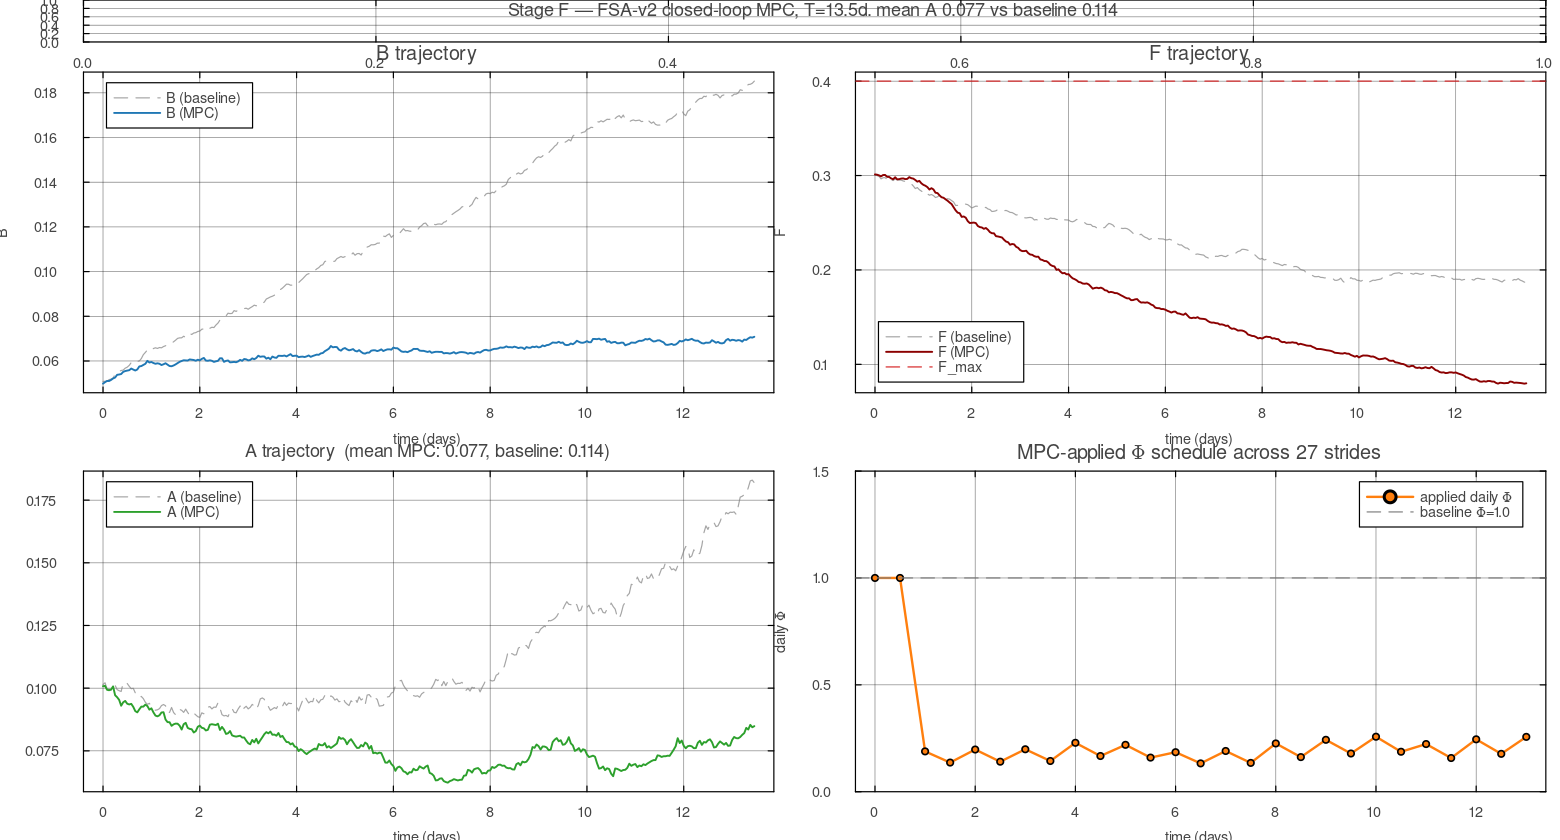
\includegraphics[width=\linewidth]{../T14d_seed42/v15_T14d_traces.png}
\caption{$T = 14$ days. State trajectories.}
\label{fig:traces_T14}
\end{figure}

\begin{figure}[ht]
\centering
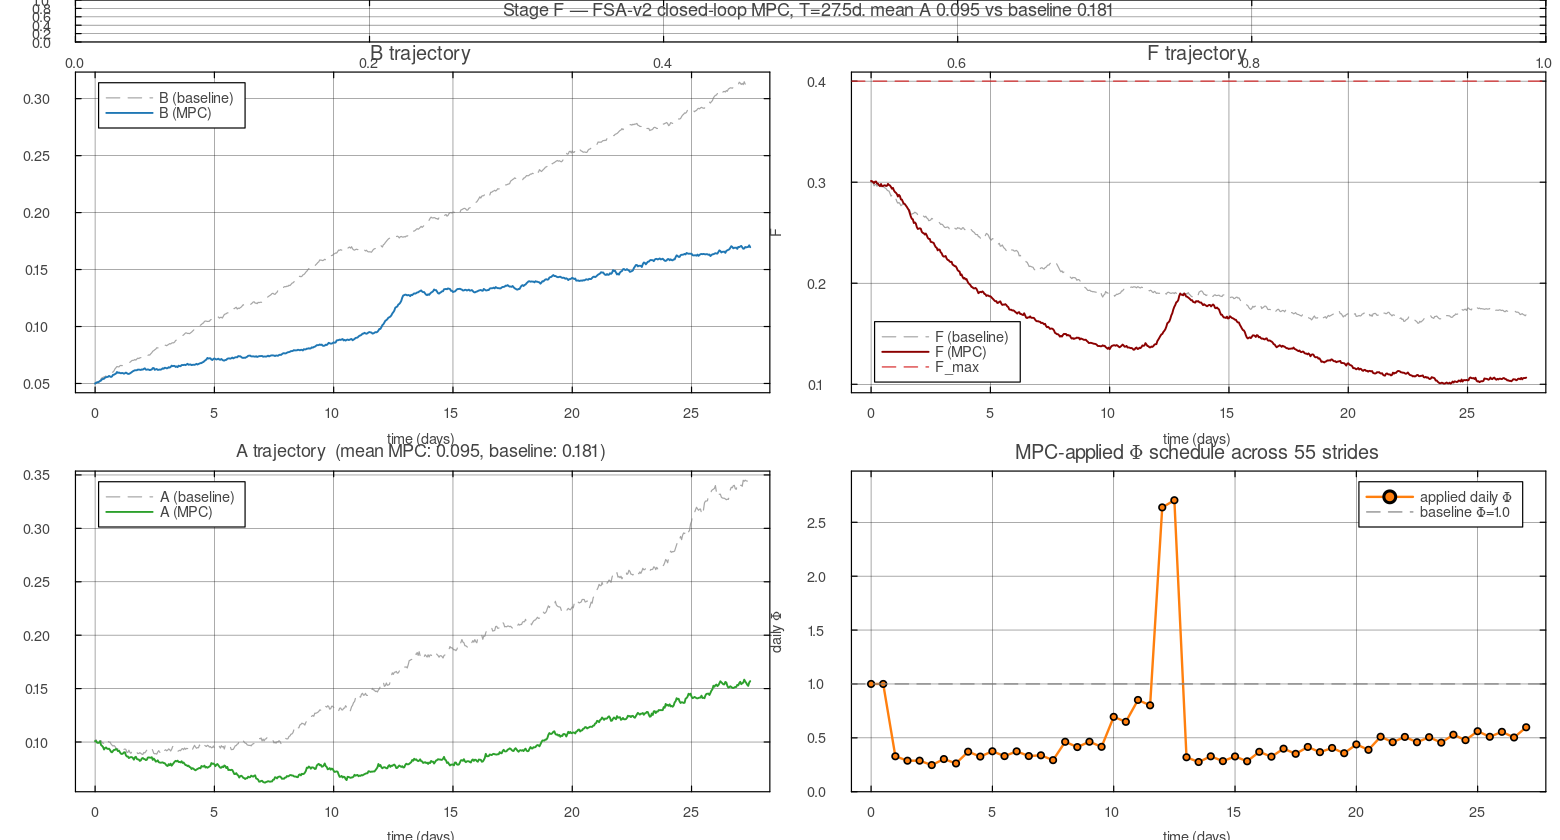
\includegraphics[width=\linewidth]{../T28d_seed42/v15_T28d_traces.png}
\caption{$T = 28$ days. State trajectories.}
\label{fig:traces_T28}
\end{figure}

\begin{figure}[ht]
\centering
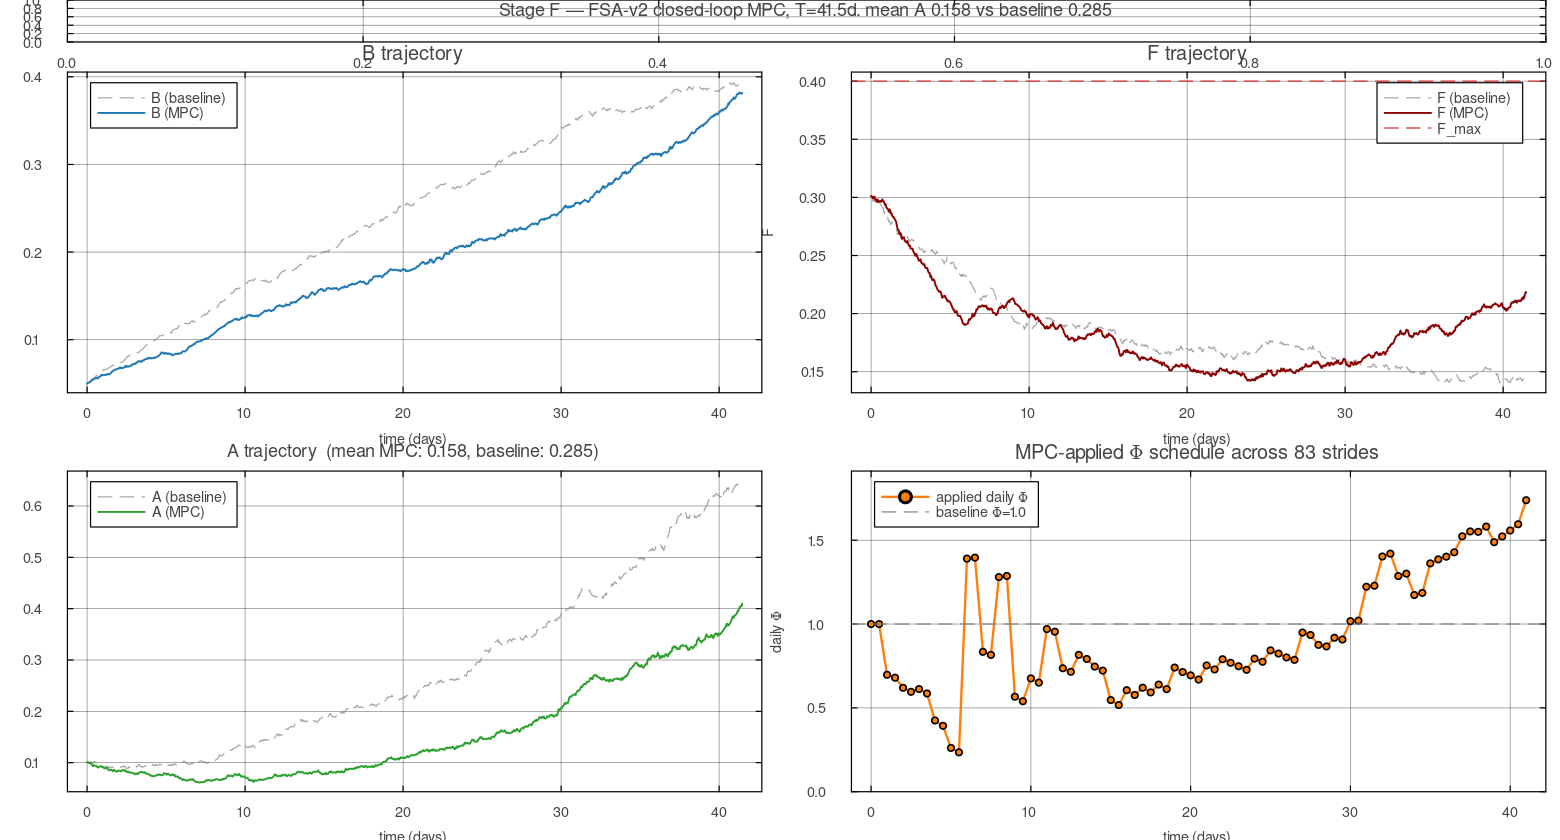
\includegraphics[width=\linewidth]{../T42d_seed42/v15_T42d_traces.png}
\caption{$T = 42$ days. State trajectories.}
\label{fig:traces_T42}
\end{figure}

\begin{figure}[ht]
\centering
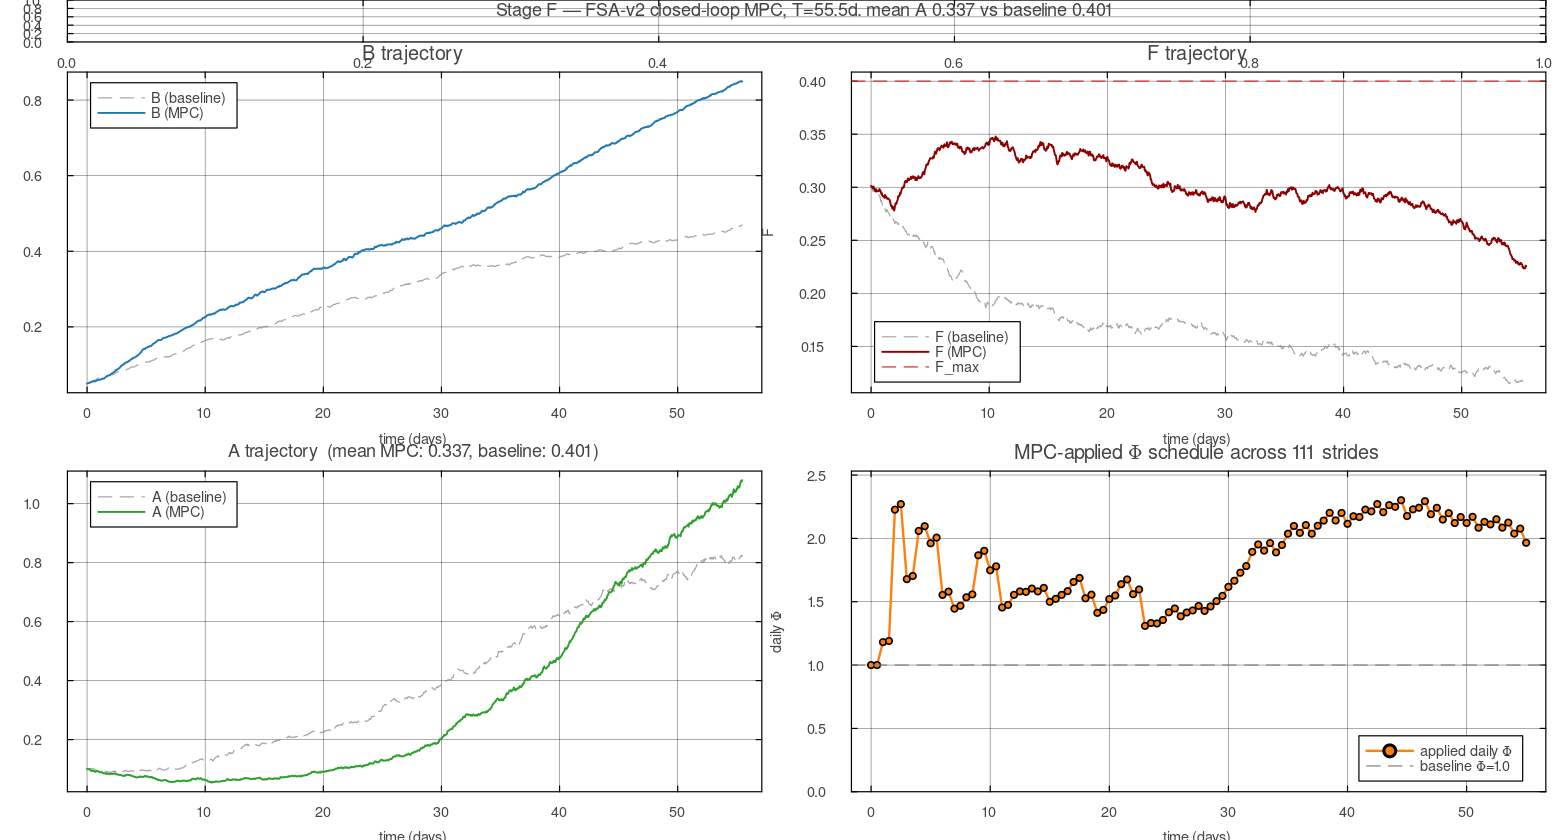
\includegraphics[width=\linewidth]{../T56d_seed42/v15_T56d_traces.png}
\caption{$T = 56$ days. State trajectories.}
\label{fig:traces_T56}
\end{figure}

\begin{figure}[ht]
\centering
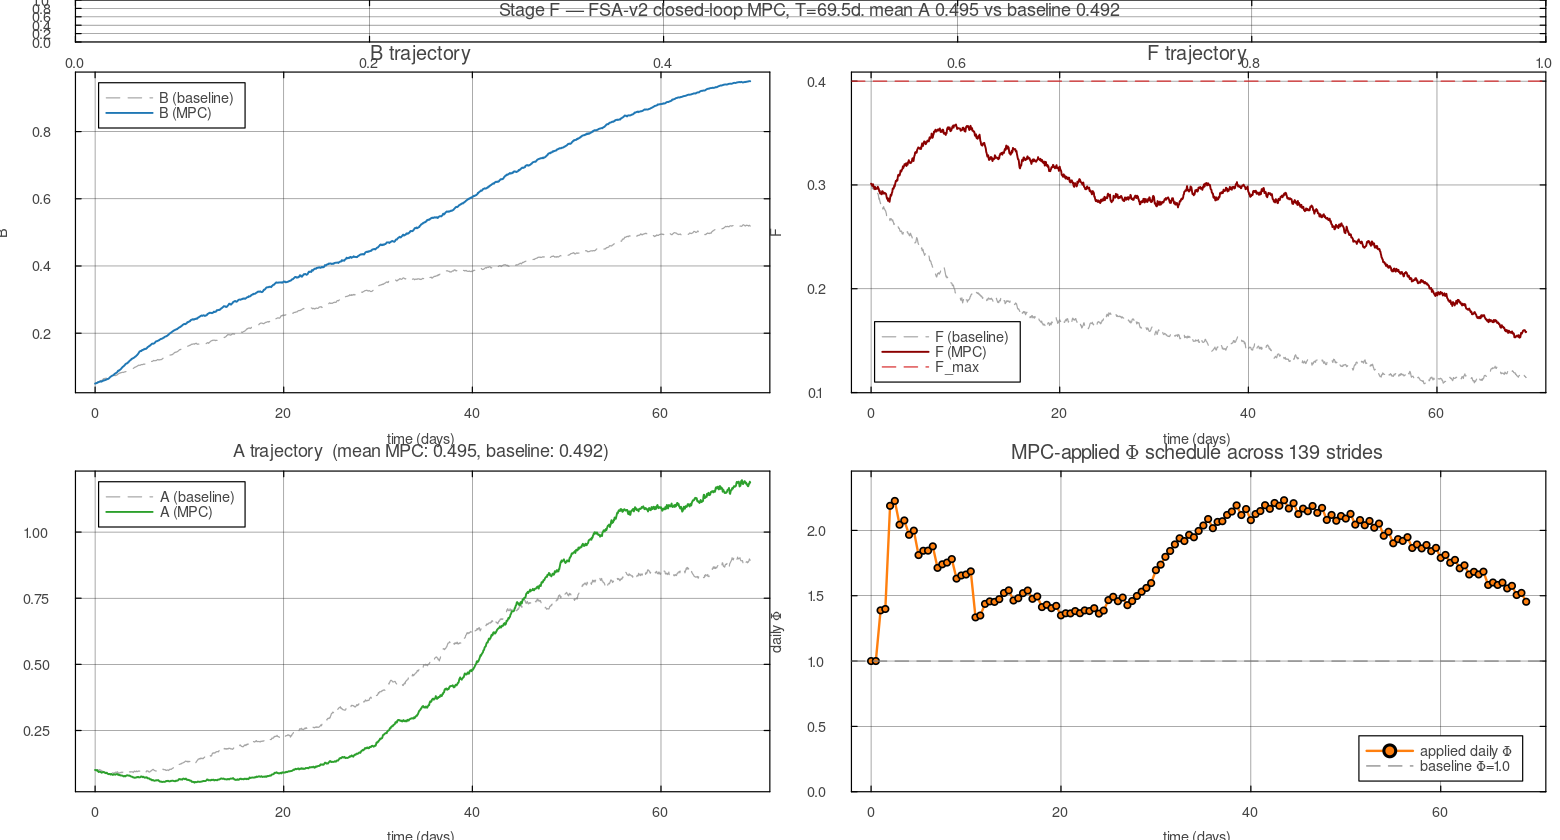
\includegraphics[width=\linewidth]{../T70d_seed42/v15_T70d_traces.png}
\caption{$T = 70$ days. State trajectories.}
\label{fig:traces_T70}
\end{figure}

\begin{figure}[ht]
\centering
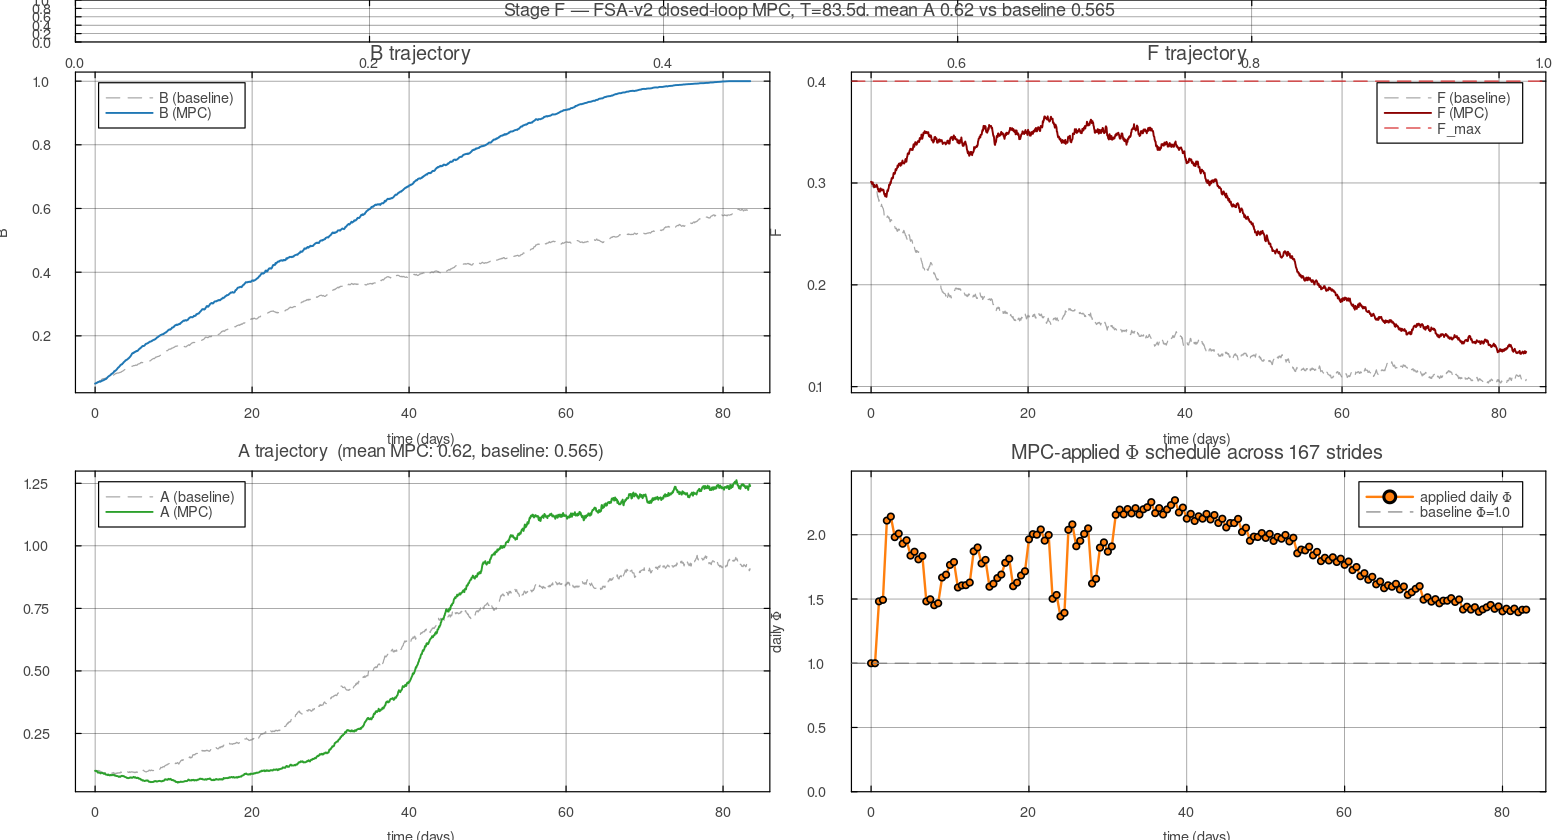
\includegraphics[width=\linewidth]{../T84d_seed42/v15_T84d_traces.png}
\caption{$T = 84$ days. State trajectories.}
\label{fig:traces_T84}
\end{figure}

\clearpage


% =====================================================================
\section{Posterior parameter traces}
\label{sec:params}

10-panel parameter-traces plot per horizon: per-parameter posterior
median (blue line) plus 5--95\% quantile band (light-blue
fill) plus truth value (red dashed line), $x$-axis in days.
Source: each horizon's \texttt{v15\_T<N>d\_param\_traces.png}.

\begin{figure}[ht]
\centering
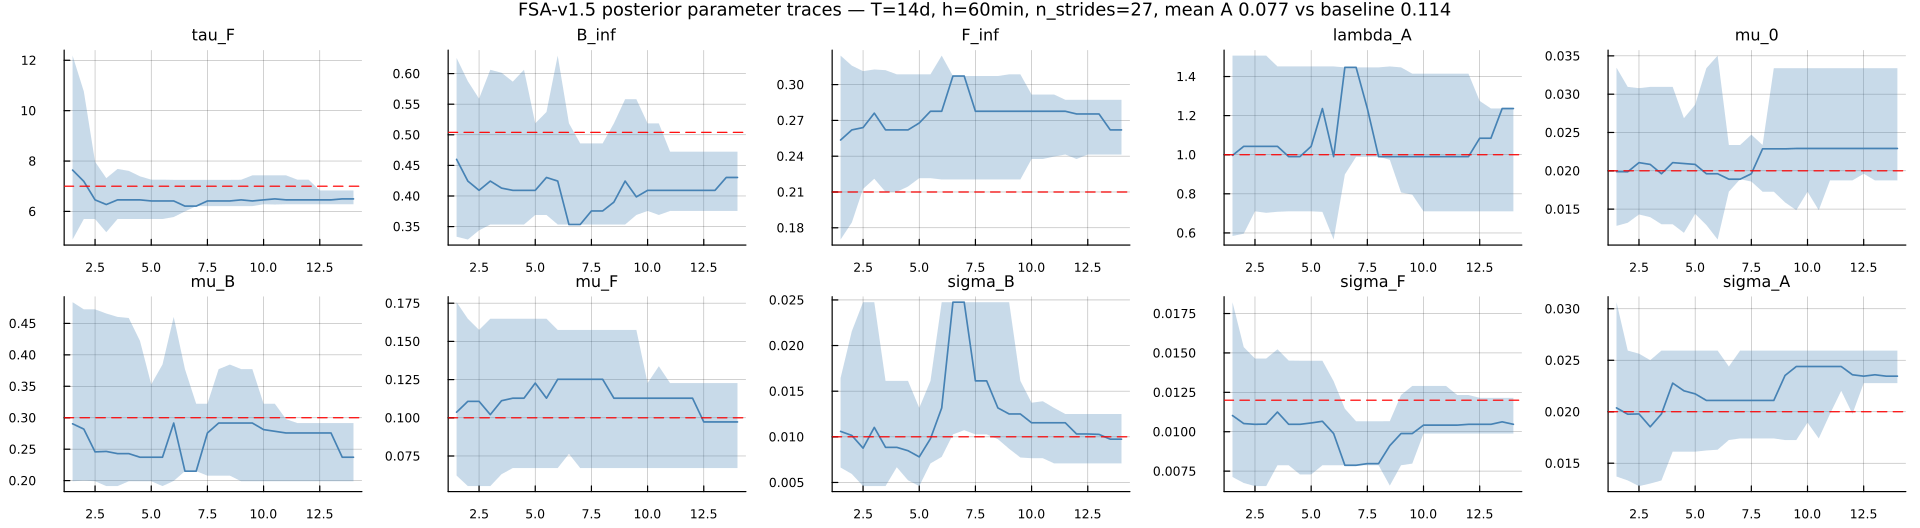
\includegraphics[width=\linewidth]{../T14d_seed42/v15_T14d_param_traces.png}
\caption{$T = 14$ days. Posterior parameter traces.}
\label{fig:param_T14}
\end{figure}

\begin{figure}[ht]
\centering
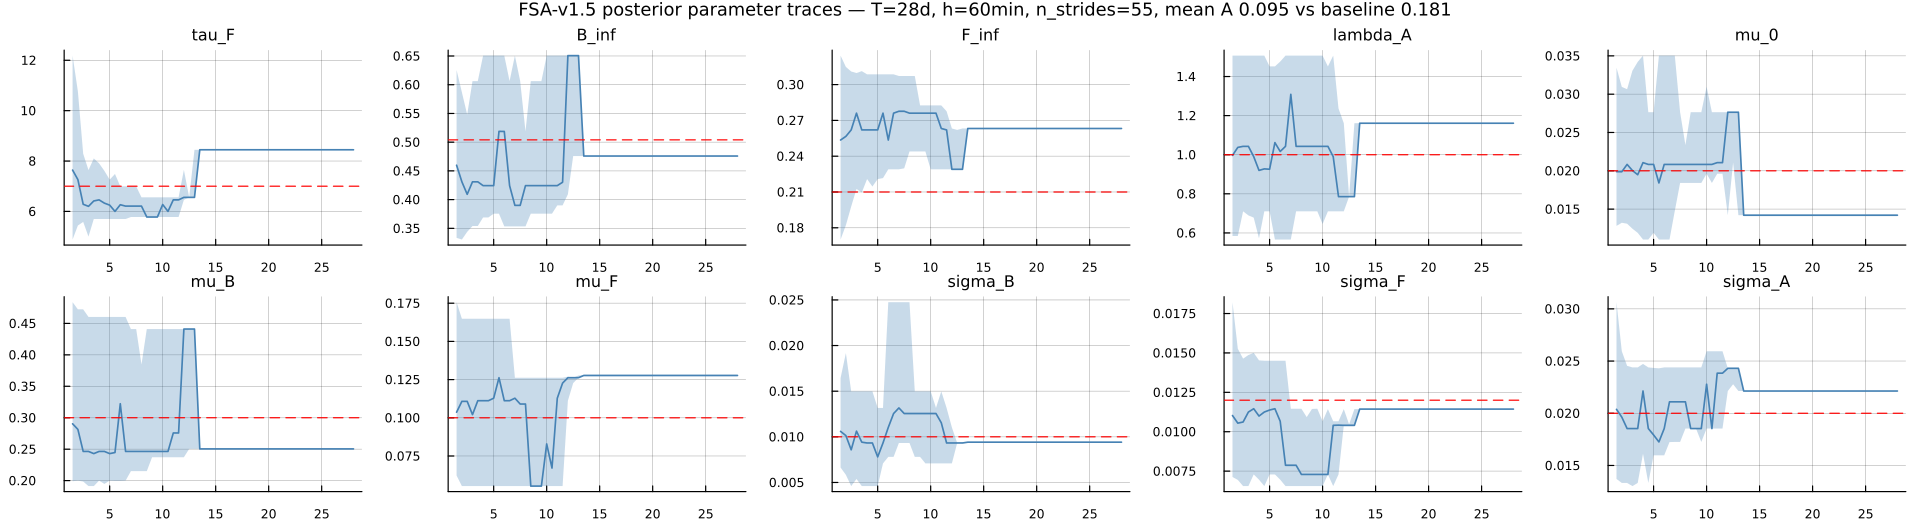
\includegraphics[width=\linewidth]{../T28d_seed42/v15_T28d_param_traces.png}
\caption{$T = 28$ days. Posterior parameter traces.}
\label{fig:param_T28}
\end{figure}

\begin{figure}[ht]
\centering
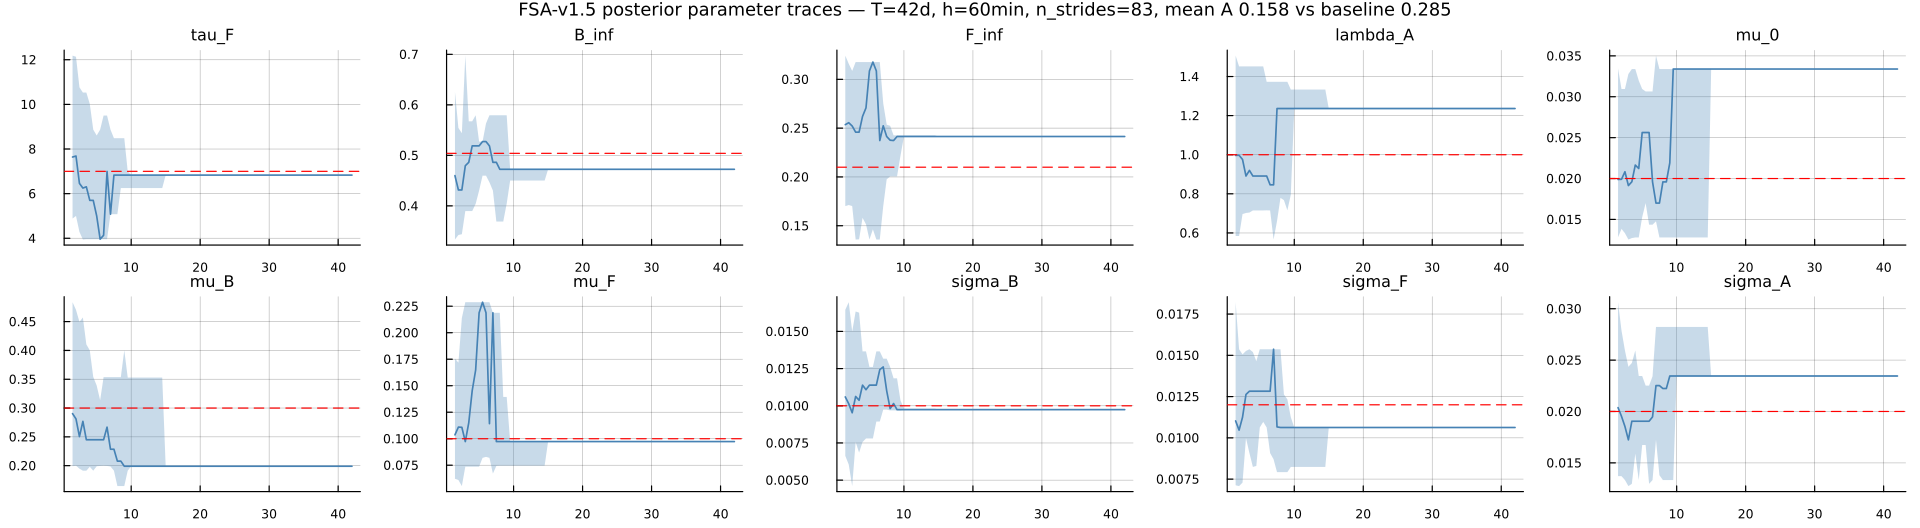
\includegraphics[width=\linewidth]{../T42d_seed42/v15_T42d_param_traces.png}
\caption{$T = 42$ days. Posterior parameter traces.}
\label{fig:param_T42}
\end{figure}

\begin{figure}[ht]
\centering
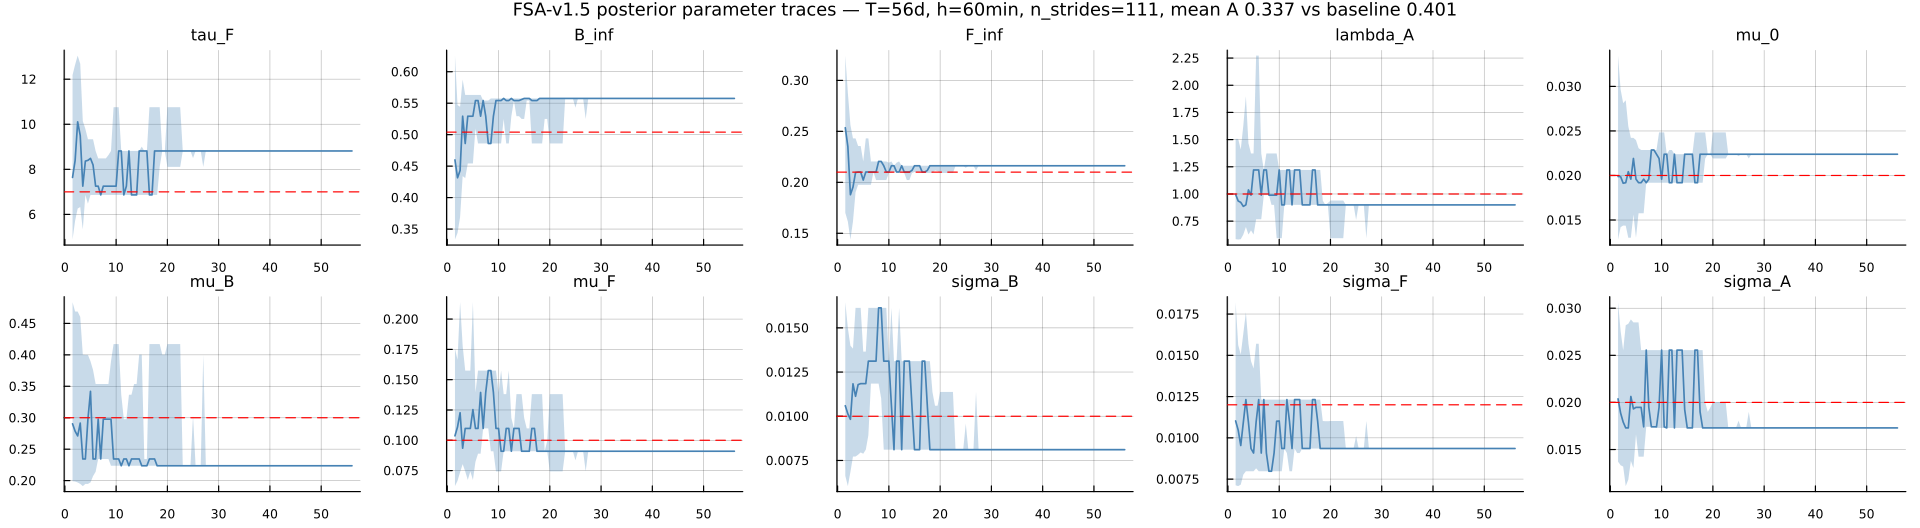
\includegraphics[width=\linewidth]{../T56d_seed42/v15_T56d_param_traces.png}
\caption{$T = 56$ days. Posterior parameter traces.}
\label{fig:param_T56}
\end{figure}

\begin{figure}[ht]
\centering
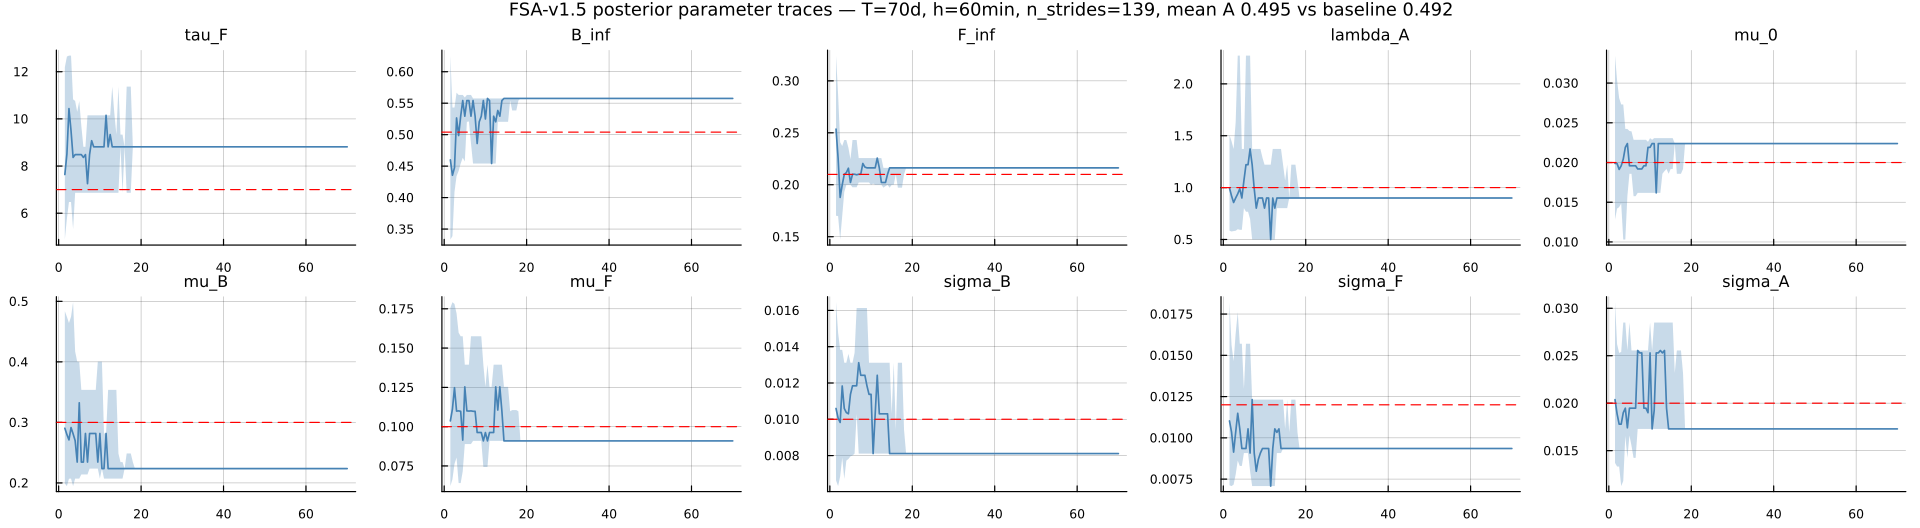
\includegraphics[width=\linewidth]{../T70d_seed42/v15_T70d_param_traces.png}
\caption{$T = 70$ days. Posterior parameter traces.}
\label{fig:param_T70}
\end{figure}

\begin{figure}[ht]
\centering
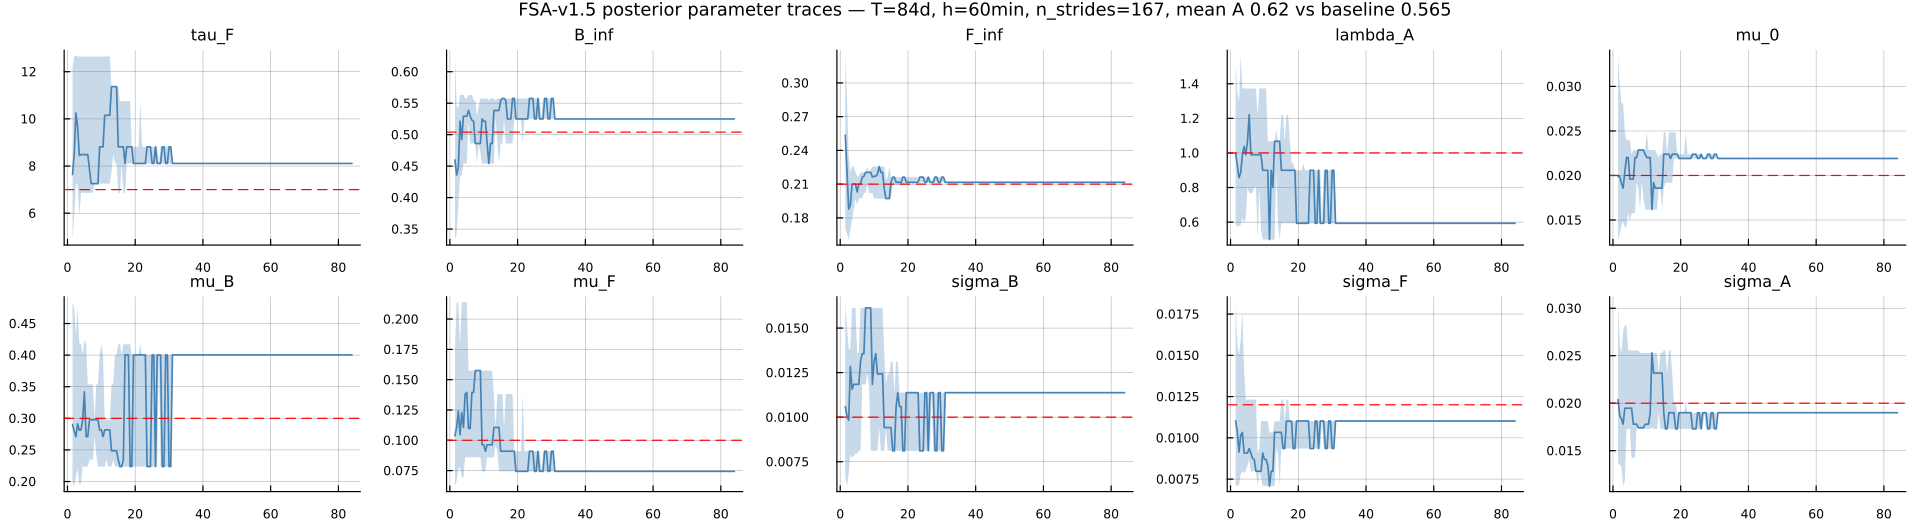
\includegraphics[width=\linewidth]{../T84d_seed42/v15_T84d_param_traces.png}
\caption{$T = 84$ days. Posterior parameter traces.}
\label{fig:param_T84}
\end{figure}

\clearpage


% =====================================================================
\appendix
\section{Agent plan (verbatim)}
\label{app:plan}

The plan that drove this sweep, archived at
\texttt{claude\_plans/Julia\_v1\_5\_multi\_horizon\_sweep\_T\_14\_to\_84\_d\_2026-05-09\_0033.md}:

\lstinputlisting[basicstyle=\ttfamily\scriptsize,breaklines=true,
                 columns=fullflexible,
                 frame=single,framerule=0pt,
                 backgroundcolor=\color{black!4}]
                {../../../../claude_plans/Julia_v1_5_multi_horizon_sweep_T_14_to_84_d_2026-05-09_0033.md}


% =====================================================================
\begin{thebibliography}{9}
\bibitem{writeup}
  \emph{FSA v1.5 closed-loop SMC$^2$-MPC: a side-by-side Python+JAX vs
  Julia comparison study.} 2026-05-08.
  \url{compare_v15_julia_vs_python/docs/julia_vs_python_v15_writeup.pdf}.
\bibitem{techguide}
  \emph{Current best Julia v1.5 SMC$^2$-FC config (RTX 5090, T=28d).}
  2026-05-08.
  \url{compare_v15_julia_vs_python/docs/technical_guide_to_current_best_Julia_SMC2FC_config.pdf}.
\end{thebibliography}

\end{document}
